\chapter{Phrase Based Machine Translation}
\section{Motivation}
Phrase based Machine Translation is another paradigm of Machine Translation which has been extremely efficient in terms of efficiency and correctness. There are certain reasons behind the rise of Phrase Based Machine Translation like
\begin{itemize}
\item Translating each word and aligning all the translated words makes the model too complicated. Sometimes, the alignment is not fully correct. PBMT systems learns the translation of phrases all-to-gather.
\item Sometimes, a word can translate into one or more words. Word-based alignment models does not model this phenomena very well.
\end{itemize}
\begin{table}[!h]
\centering
	\caption{English Phrase and its translated Hindi Phrases}
    \label{table:phrase}
	\begin{tabular}{c c c}
    \hline
    Number & Hindi Word Sequence & Probability \\
    \hline
    1 & \begin{hindi} भारत के प्रधान मंत्री \end{hindi} & 0.75 \\
    2 & \begin{hindi} भारत के भूतपूर्व प्रधान मंत्री  \end{hindi} & 0.02 \\
    3 & \begin{hindi} प्रधान मंत्री \end{hindi} & 0.23 \\
    \hline
	\end{tabular}
\end{table}

Table \ref{table:phrase} shows an example\cite{bhattacharyya} of English phrase `Prime Minister of India' and sample Hindi translated phrase with their probability. It has to be noted that, Phrases and their translation can be both linguistic and Non-linguistic. Table \ref{table:phrase2} shows some example of linguistic and non-linguistic phrases. 

\begin{table}[H]
\centering
	\caption{Linguistic and Non-linguistic Phrase}
    \label{table:phrase2}
	\begin{tabular}{c c c c}
    \hline
    Number & English Word Sequence & Hindi Word Sequence & Phrase Type\\
    \hline
    1 & Near Yamuna river & \begin{hindi} यमुना किनारे \end{hindi} & non-linguistic phrase\\
    2 & Where are you & \begin{hindi}किधर हो \end{hindi} & linguistic phrase \\
    3 & See you again & \begin{hindi} फिर मिलेंगे  \end{hindi} & linguistic phrase \\
    4 & It's tough & \begin{hindi} यह मुश्किल है   \end{hindi} & linguistic phrase\\
    \hline
	\end{tabular}
\end{table}

\section{Phrase Alignment Technique}
Phrases are constructed from sentence using following steps.
\subsection{Alignment Between Sentences}
For any pair of sentence between source and target language, words of sentence are aligned to form a tuple. Figure \ref{fig:hindi_english} and Figure \ref{fig:english_hindi} shows alignment from Hindi to English and English to Hindi sentence. 

\begin{figure}[H]
        \centering
        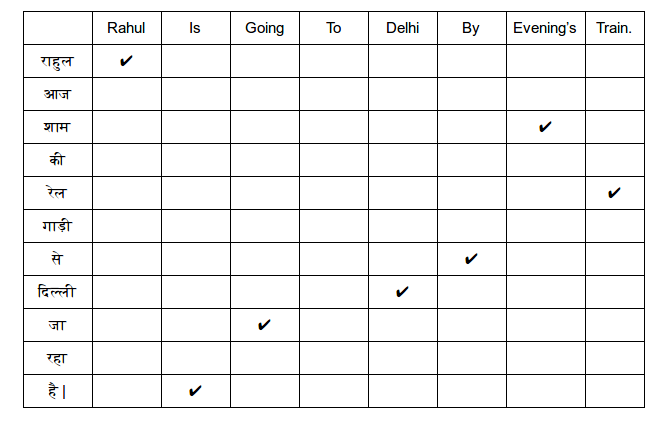
\includegraphics[scale=0.4]{Images/hindi_english}
        \caption{Alignment from Hindi to English}
        \label{fig:hindi_english}
\end{figure}
 A cell has \checkmark symbol if the row and column word are translation of each other. It is also possible that an entire row or column will not have \checkmark symbol, that's because there is no translation of that word in entire sentence. This is usually true for Articles and filler words.
\begin{figure}[H]
        \centering
        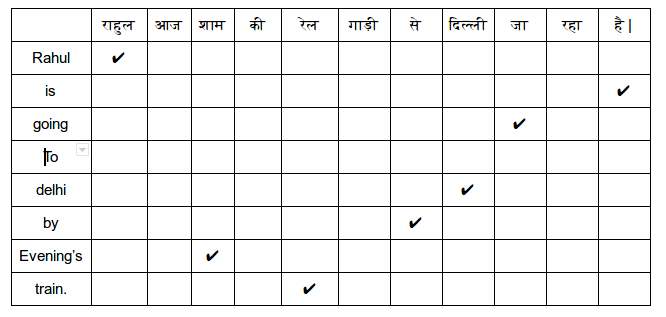
\includegraphics[scale=0.4]{Images/english_hindi}
        \caption{Alignment from English to Hindi}
        \label{fig:english_hindi}
\end{figure}
\subsection{Phrase construction}
Given word alignments, phrases are constructed as follows\cite{bhattacharyya,koehn}:
\begin{enumerate}
\item Every word of the sentence must be in some phrase.(Principle of coverage)
\item No empty phase is allowed. (Principal of Non-vacuousness).
\item All the words of language $L_{1}$ involved in a phrase must only align with words of language $L_{2}$ of the same phrase. (Principal of consistency)
\end{enumerate}
Figure \ref{fig:boxed} shows a possible phrases formed from the alignment phrases. Note that any given box will always follow the three principles of phrase construction. Figure \ref{fig:boxed_complete} shows bigger phrases formed using the  alignment figures \ref{fig:hindi_english} and \ref{fig:english_hindi}.
\begin{figure}[H]
        \centering
        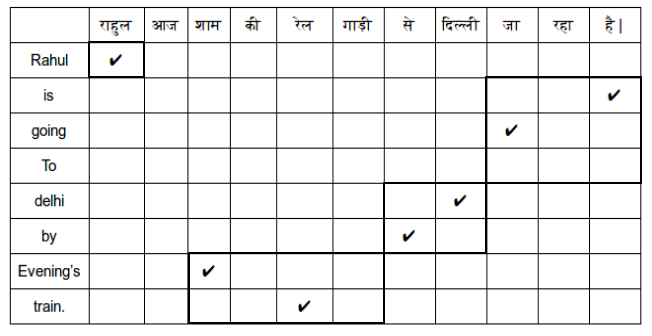
\includegraphics[scale=0.4]{Images/boxed.png}
        \caption{Few possible phrases from Alignments in figure \ref{fig:hindi_english} and \ref{fig:english_hindi}}
        \label{fig:boxed}
\end{figure}
\begin{figure}[H]
        \centering
        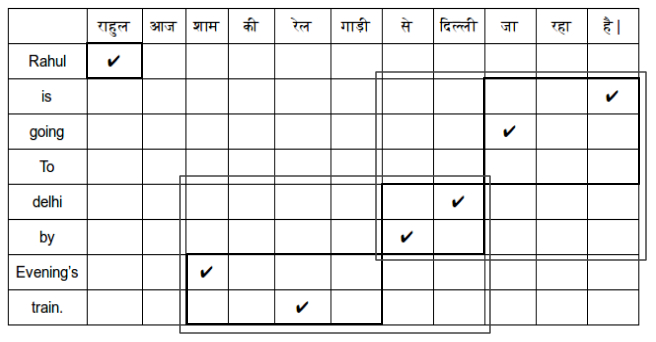
\includegraphics[scale=0.4]{Images/boxed_complete.png}
        \caption{Larger Phrases formed from figure \ref{fig:hindi_english} and \ref{fig:english_hindi}}
        \label{fig:boxed_complete}
\end{figure}

\section{Phrase Based SMT}
Phrase based SMT follows the same Noisy-channel model as
\begin{equation}
\hat{e} = arg max_{e}(P(e\mid f)) = arg max_{e}(P(e)\cdot(f\mid e))
\end{equation}
\begin{align}
P(f_{1}^{I}\mid e_{1}^{I}) &= P(f_{1},f_{2},\ldots,f_{I}\mid  e_{1},e_{2},\ldots,e_{I})\nonumber \\
		   &= \prod_{i=1}^{I}\Phi(f_{i}^{I}\mid e_{i}^{I})d(start_{i}-end{(i-1)}-1)
\end{align}

where LHS is the probability of $I$ phrases of $f$ given $I$ phrases of $e$ and RHS consists of two parts. The first part $\Phi$ is called the phrase translation probability, while the second part $d(\cdot)$ is called the distortion probability. 

\subsection{Estimating Phrase Translation and Distortion probability }
Phrase translation probability is found out by counting in how many sentences a particular phrase pair was extracted again all possible phrases of a English phrase.
\begin{equation}
\phi(f\mid e) = \frac{count(e,f)}{\sum_{f_{i}}count(e,f_{i})}
\end{equation}
Distortion probability is found out by simply for each phrase, calculating the difference in the position of the phrase in the input and translated sentence.
\begin{equation}
d(distance) = \frac{count(distance(\bar{e},\bar{f}))}{count(\bar{e})}
\end{equation}
The two candidate translation of \begin{hindi} फिर मिलेंगे, \end{hindi} \\
See you again.\\
Again see you, \\
will be decided using following parameters.
\begin{enumerate}
\item $P_{LM}(\text{see you again})$ and $P_{LM}(\text{see you again})$\\
\item $P(milenge\mid \text{see you})$ and $P(fir\mid again)$ \\
\item Distortion probability of $see you$ and $again$. 
\end{enumerate}







